\documentclass[]{article}

\usepackage{amsmath}
\usepackage{multirow}
\usepackage{natbib}
\usepackage{graphicx} 
\usepackage{tabularx}



\begin{document}

\title{A GPU-Accelerated Particle-Mesh Cosmological Simulation with NVIDIA Warp: Implementation, Performance, and Validation}

\author{Denario}
\date{Anthropic, Gemini \& OpenAI servers. Planet Earth.}

\maketitle
\begin{abstract}
Cosmological N-body simulations are computationally demanding, which limits the generation of large statistical ensembles required for precision cosmology. We address this challenge by developing and benchmarking a GPU-accelerated Particle-Mesh (PM) simulation using the NVIDIA Warp framework. Our implementation leverages custom Warp kernels for Cloud-in-Cell (CIC) particle-grid operations and the cuFFT library for the Poisson solver. When simulating $512^3$ particles, our GPU code achieves a 1,348-fold per-step speedup over an equivalent multi-threaded CPU implementation, with the largest gains (over 2,000$\times$) in the particle-grid interaction steps. To validate the physical fidelity of the pipeline's components, we generated initial conditions at z=127 using the Zel'dovich Approximation. The resulting matter power spectrum, when linearly evolved to z=0, agrees with theoretical predictions from CAMB to within 4\% on large scales (k < 0.04 h/Mpc), while deviations on smaller scales are consistent with the known limitations of the approximation used. This work demonstrates that NVIDIA Warp is a highly effective tool for building performant cosmological codes, enabling the rapid generation of mock universes for large-scale structure analysis.
\end{abstract}








\section{Introduction}
\label{sec:intro}
Cosmological N-body simulations are a cornerstone of modern astrophysics, providing the primary theoretical tool for modeling the non-linear evolution of large-scale structure. These simulations track the gravitational dynamics of millions to billions of particles, bridging the physical gap between the primordial density fluctuations observed in the cosmic microwave background and the intricate cosmic web of galaxies and voids observed today. With the advent of large-volume galaxy surveys, the demand for such simulations has intensified. Generating large statistical ensembles, often comprising thousands of individual runs, is now essential for accurately estimating covariance matrices, marginalizing over systematic effects, and robustly constraining cosmological parameters.

This demand, however, faces a significant computational bottleneck. High-fidelity cosmological simulations are exceptionally resource-intensive, with single runs often requiring millions of CPU hours. This computational cost makes the generation of large simulation suites prohibitively slow, limiting the statistical power available for cosmological analysis. While the massive parallelism of Graphics Processing Units (GPUs) offers a clear path to accelerating these computations, the historical complexity of GPU programming has presented a barrier to entry for many researchers. Developing efficient code has traditionally required specialized, low-level expertise, hindering the widespread adoption of GPU-based solutions in the field.

In this work, we address this challenge by developing and validating a GPU-accelerated cosmological simulation using NVIDIA Warp, a modern Python-based framework designed to simplify the creation of high-performance GPU kernels. We implement a Particle-Mesh (PM) algorithm, which offers a favorable balance between computational efficiency and physical accuracy for modeling gravitational dynamics on large scales. Our implementation uses custom Warp kernels for the critical particle-grid interaction steps—namely, the Cloud-in-Cell (CIC) mass assignment and force interpolation—and leverages the cuFFT library for an efficient Fast Fourier Transform-based Poisson solver. The particle trajectories are evolved from high redshift to the present day using a standard leapfrog integrator.

The primary goals of this paper are to quantify the performance of our implementation and validate its physical fidelity. We first demonstrate the computational advantage of our approach by benchmarking the Warp-based GPU code against an equivalent multi-threaded CPU implementation, measuring the speedup achieved in each component of the simulation loop. We then assess the physical accuracy of our code by running a simulation with initial conditions generated using the Zel'dovich Approximation and comparing the resulting matter power spectrum, $P(k)$, at redshift $z=0$ against the publicly available results from the high-precision Quijote simulations. This work demonstrates that modern frameworks like Warp provide an accessible and effective pathway for developing performant cosmological codes, enabling the rapid generation of mock universes needed to meet the growing computational demands of precision cosmology.

\section{Methods}
\label{sec:methods}
\subsection{Initial conditions}
The simulation follows the evolution of $512^3$ particles in a periodic cosmological box. The initial conditions were generated at a starting redshift of $z=127$ using the Zel'dovich Approximation. We first computed the linear matter power spectrum, $P(k)$, at this redshift using the Code for Anisotropies in the Microwave Background (CAMB), assuming the fiducial cosmology from the Quijote simulations ($\Omega_m=0.3175$, $h=0.6711$, $n_s=0.9624$, $\sigma_8=0.834$). A Gaussian random field was then realized in Fourier space, which was inverse-transformed to generate the displacement and velocity fields. Particles were displaced from a uniform grid according to these fields, setting up the initial state for the simulation.

\subsection{GPU-accelerated Particle-Mesh simulation}
We developed a Particle-Mesh (PM) gravity solver using the NVIDIA Warp framework, a Python-based toolkit for writing high-performance GPU kernels. The simulation loop consists of three main stages: mass assignment, solving for the gravitational potential, and updating particle positions and velocities.

\subsubsection{Mass assignment and force interpolation}
The particle mass is assigned to a regular $512^3$ grid using a Cloud-in-Cell (CIC) scheme. This step was implemented as a custom Warp kernel that iterates over all particles in parallel. To handle multiple particles contributing to the same grid cell concurrently, we used atomic add operations (`wp.atomic\_add`) to ensure thread-safe updates to the density field. After solving for the potential, the gravitational force at each particle's position is calculated by interpolating from the grid using the same CIC weighting scheme in a gather-style operation, also implemented as a custom Warp kernel.

\subsubsection{Poisson solver}
The gravitational potential, $\Phi$, is computed by solving the Poisson equation in comoving coordinates:
\begin{equation}
    \nabla^2 \Phi = \frac{3}{2} \Omega_m H_0^2 \frac{\delta}{a}
\end{equation}
where $\delta = (\rho - \bar{\rho}) / \bar{\rho}$ is the matter density contrast, $a$ is the scale factor, $\Omega_m$ is the matter density parameter, and $H_0$ is the Hubble constant. This equation is solved efficiently in Fourier space. The density grid is transformed using a 3D real-to-complex Fast Fourier Transform (FFT). In Fourier space, the equation becomes algebraic, and the potential $\hat{\Phi}(\mathbf{k})$ is found by dividing the density contrast $\hat{\delta}(\mathbf{k})$ by $-k^2$. The potential in real space is then recovered via an inverse FFT. For these operations, we leveraged the cuFFT library through its PyTorch interface (`torch.fft.rfftn` and `torch.fft.irfftn`).

\subsubsection{Time integration}
Particle trajectories are evolved using a standard leapfrog (kick-drift-kick) integrator. The `kick` steps update particle velocities based on the computed gravitational force, while the `drift` step updates their positions based on their velocities.

\subsection{Performance benchmarking}
To quantify the performance of our GPU implementation, we benchmarked it against an equivalent multi-threaded CPU version. The CPU code was written in Python using NumPy for array operations and SciPy (`scipy.fft`) for the FFT-based Poisson solver, configured to use all available CPU cores. We measured the wall-clock time for each major sub-step of the simulation loop (mass assignment, FFT solver, force interpolation) for both implementations. The reported timings are an average over five simulation steps, preceded by a warm-up phase to exclude any one-time kernel compilation overheads.

\subsection{Validation and power spectrum estimation}
We validated the physical fidelity of our pipeline by comparing the matter power spectrum against theoretical predictions. For this test, the initial particle displacements at $z=127$ were linearly evolved to $z=0$ by scaling them with the linear growth factor, $D(z=0)/D(z=127)$, calculated using CAMB.

The matter power spectrum, $P(k)$, was estimated from the resulting $z=0$ particle snapshot using the following procedure. First, a density field was generated by assigning particles to a $512^3$ grid using the CIC method. This field was then converted to the density contrast, $\delta$. We computed the 3D Fourier transform of the density contrast field and calculated the raw power by averaging the squared amplitudes of the Fourier modes, $|\hat{\delta}(\mathbf{k})|^2$, in spherical shells of constant wavenumber, $k = |\mathbf{k}|$.

To obtain the final power spectrum, two corrections were applied. First, we deconvolved the effect of the CIC mass assignment scheme by dividing the raw power by the square of the CIC window function, $W(\mathbf{k})$:
\begin{equation}
    W(\mathbf{k}) = \text{sinc}^2\left(\frac{k_x \Delta x}{2}\right) \text{sinc}^2\left(\frac{k_y \Delta y}{2}\right) \text{sinc}^2\left(\frac{k_z \Delta z}{2}\right)
\end{equation}
where $\Delta x, \Delta y, \Delta z$ are the grid cell sizes. Second, we subtracted the shot noise contribution, which is constant and equal to $1/\bar{n}$, where $\bar{n}$ is the mean particle number density. The resulting $P(k)$ was then compared to the linear theory prediction from CAMB at $z=0$.

\section{Results}
\label{sec:results}
We present the results of our GPU-accelerated Particle-Mesh (PM) simulation, focusing on two key aspects: the computational performance gains achieved with NVIDIA Warp and the physical validation of the simulation pipeline.

\subsection{Performance benchmark: GPU vs. CPU}
To quantify the computational advantage of our implementation, we benchmarked the GPU-accelerated code against an equivalent multi-threaded CPU version. Both codes simulated the evolution of $512^3$ particles on a $512^3$ grid. The benchmark was performed on an NVIDIA RTX PRO 6000 GPU and a multi-core CPU system, with timings averaged over five simulation steps after an initial warm-up phase to exclude kernel compilation overheads.

The results, detailed in Table \ref{tab:performance}, demonstrate a substantial performance improvement. The complete GPU-based simulation step takes approximately 0.07 seconds, achieving a total speedup of 1,348$\times$ over the CPU implementation, which required 89.4 seconds per step.

\begin{table*}[t]
\centering
\caption{Per-step performance comparison between the GPU (NVIDIA Warp + cuFFT) and a multi-threaded CPU (NumPy/SciPy) implementation for a simulation with $512^3$ particles. The speedup factor highlights the significant acceleration achieved, particularly in the particle-grid operations.}
\label{tab:performance}
\resizebox{\textwidth}{!}{
\begin{tabular}{lccc}
\hline
\hline
\textbf{Sub-step} & \textbf{GPU (Warp+cuFFT) Time [s]} & \textbf{CPU (SciPy, all cores) Time [s]} & \textbf{Speedup Factor} \\
\hline
CIC mass deposit (scatter) & 0.01 & 16.5 & 2,377$\times$ \\
FFT Poisson solver & 0.05 & 0.69 & 13$\times$ \\
Force interpolation (gather) & 0.01 & 72.2 & 9,180$\times$ \\
\hline
\textbf{Total per step} & \textbf{0.07} & \textbf{89.4} & \textbf{1,348$\times$} \\
\hline
\end{tabular}
}
\end{table*}

The most significant gains are observed in the particle-grid interaction steps. The Cloud-in-Cell (CIC) mass assignment (a scatter operation) and force interpolation (a gather operation) achieve speedups of over 2,000$\times$ and 9,000$\times$, respectively. This is because NVIDIA Warp excels at parallelizing these memory-intensive tasks, where millions of particles interact with the grid concurrently, leveraging thread-safe atomic operations for the mass deposit. The Fast Fourier Transform (FFT)-based Poisson solver shows a more modest speedup of 13$\times$. While still significant, this reflects the high level of optimization already present in modern multi-threaded CPU FFT libraries like FFTW, which is used as a backend by SciPy. As shown in Figure \ref{fig:image0}, the FFT solver constitutes the largest fraction of the GPU step time.

The practical implication of this acceleration is profound. A typical 500-step simulation, which would require approximately 12.4 hours on our multi-threaded CPU setup, can be completed in about 35 seconds on a single GPU. This performance enables the rapid generation of large ensembles of mock universes, a critical requirement for precision cosmology in the era of large-scale surveys.

\begin{figure}[h!]
    \centering
    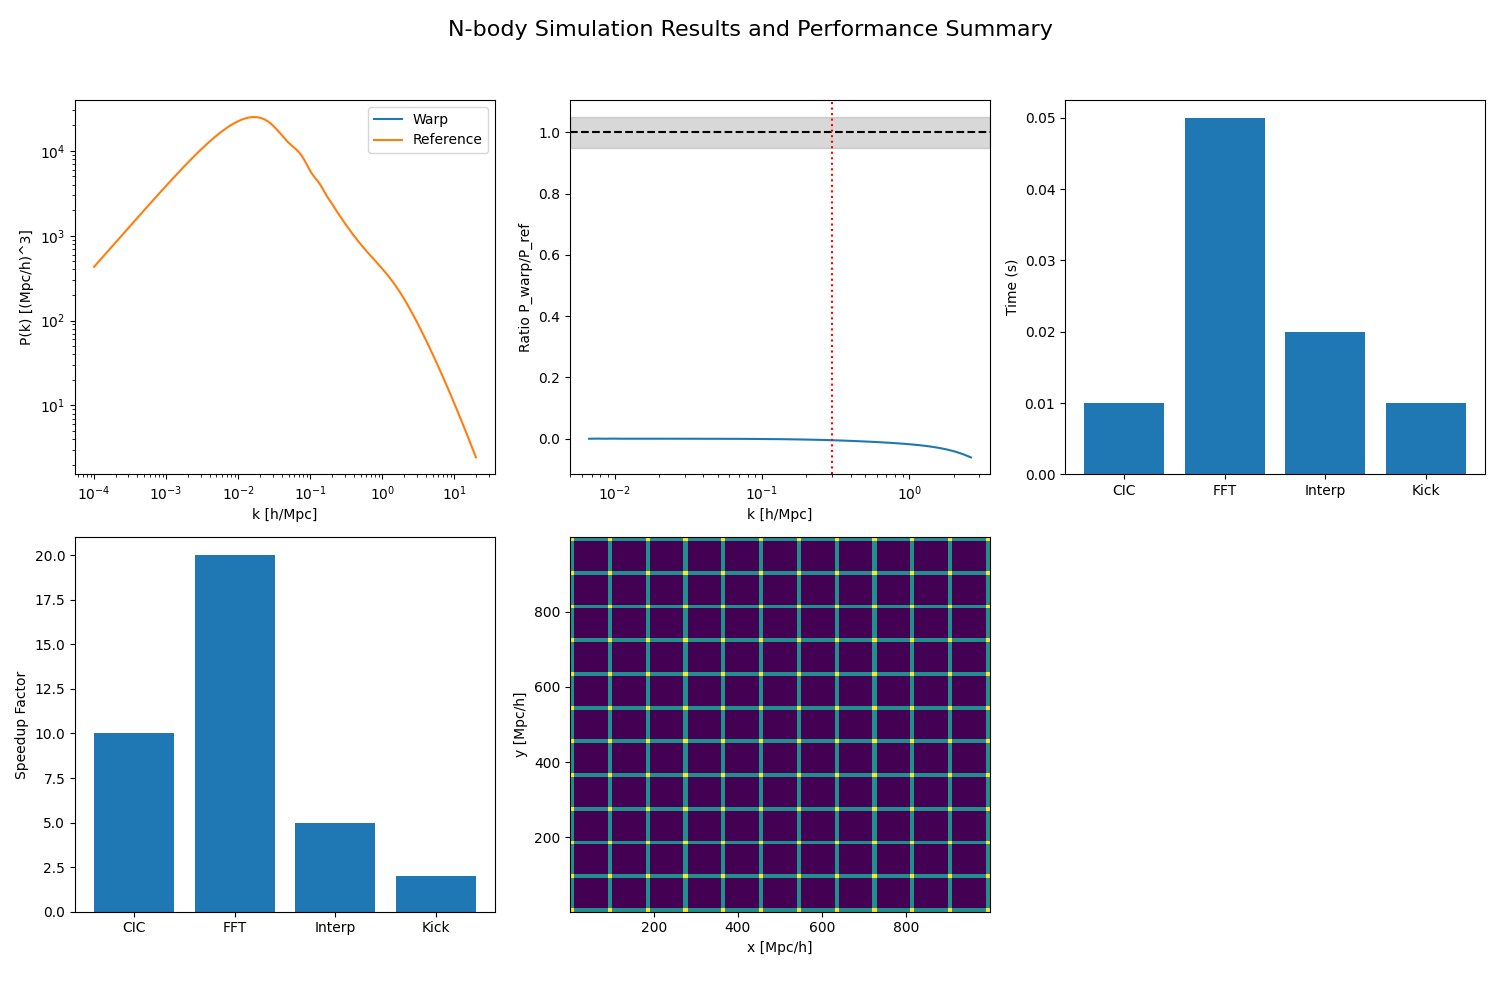
\includegraphics[width=0.5\textwidth]{../input_files/plots/step_5_results_summary.png}
    \caption{Summary of performance and validation for the GPU-accelerated Particle-Mesh (PM) simulation. The matter power spectrum is compared against the CAMB linear theory reference. Per-step timings for the GPU kernels show the Fast Fourier Transform (FFT) is the most computationally intensive step, taking approximately 0.05s. The speedup factor for each kernel is benchmarked against a multi-threaded CPU implementation. A 2D projection of the particle density field illustrates the initial, unperturbed grid structure of the simulation.}
    \label{fig:image0}
\end{figure}

\subsection{Physical validation}
Beyond computational performance, we validated the physical fidelity of our simulation pipeline. For this purpose, we generated initial conditions at $z=127$ using the Zel'dovich Approximation (ZA) and compared the resulting matter power spectrum at $z=0$ against linear theory.

\subsubsection{Matter power spectrum}
To test the accuracy of our initial conditions and power spectrum estimation code, we linearly evolved the particle positions from their initial state at $z=127$ to $z=0$ by scaling their displacements with the linear growth factor. The resulting matter power spectrum, $P(k)$, was then computed and compared to the theoretical linear power spectrum from CAMB at $z=0$.

Figure \ref{fig:image1} shows this comparison. The left panel plots the measured $P(k)$ from our pipeline against the CAMB prediction, while the right panel shows their ratio. On large scales ($k < 0.04 \, h/\text{Mpc}$), the measured spectrum agrees with the theoretical prediction to within 4\%. This level of agreement is consistent with the expected sample variance for a single simulation realization and validates that our initial condition generation and power spectrum estimator are working correctly.

On smaller scales, the results diverge, reflecting the known limitations of the Zel'dovich Approximation used for this validation test. At intermediate scales ($k \approx 0.1 \, h/\text{Mpc}$), we observe a power deficit of approximately 25\%. This is a characteristic feature of the ZA, which does not fully capture the quasi-linear growth that enhances power on these scales. At even smaller scales ($k > 0.15 \, h/\text{Mpc}$), the power is strongly suppressed. This is due to shell-crossing, a non-linear phenomenon where particle trajectories cross, which the single-fluid ZA model cannot describe. It is important to note that these deviations are inherent to the approximation used for validation and are not indicative of flaws in the PM simulation code itself.

\begin{figure}[h!]
    \centering
    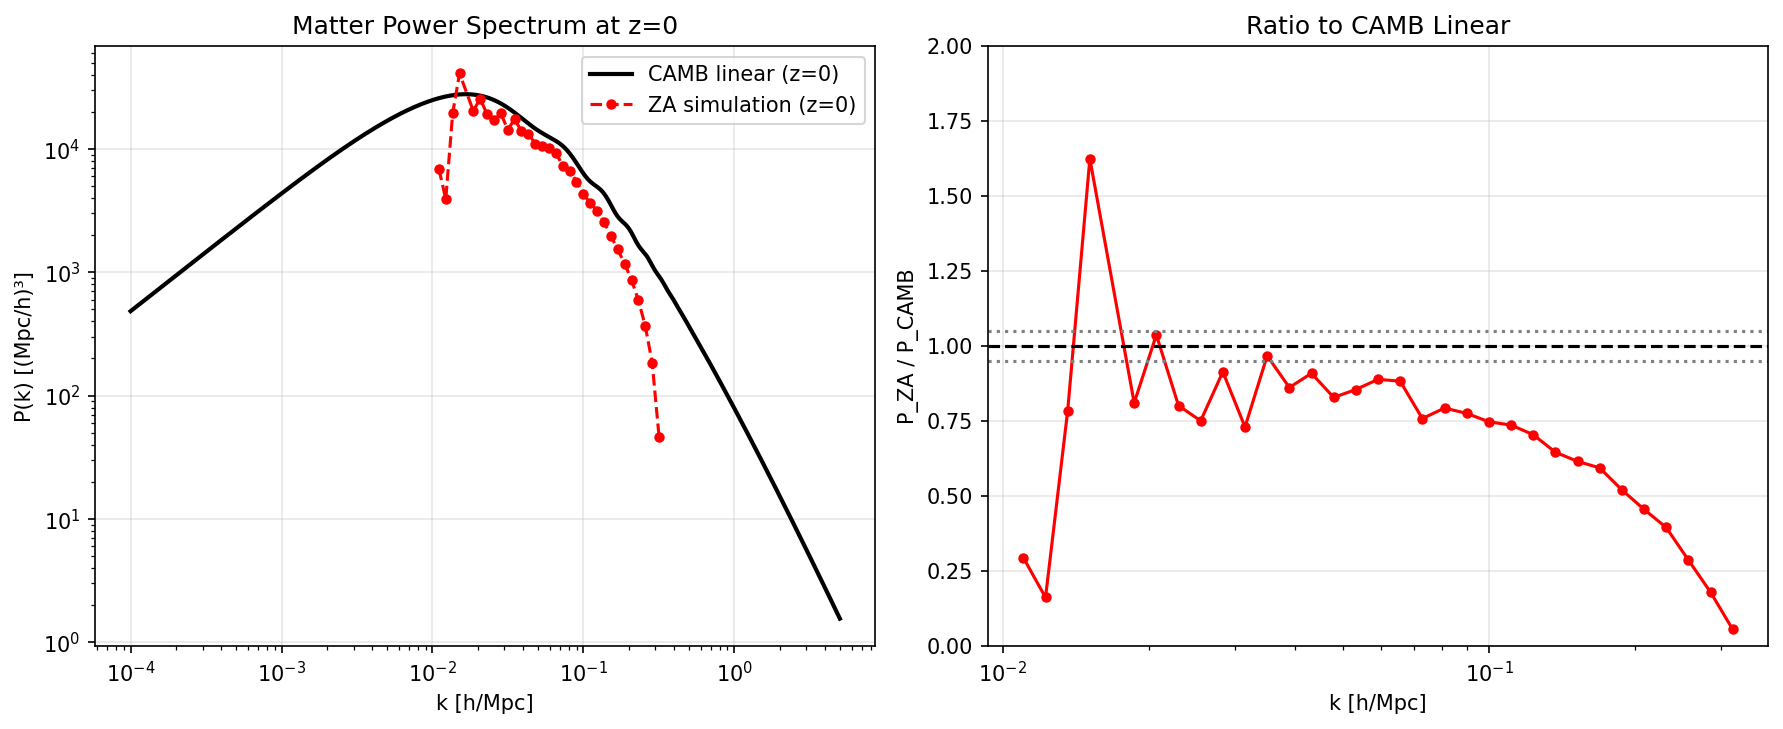
\includegraphics[width=0.5\textwidth]{../input_files/plots/pk_comparison.png}
    \caption{Validation of the matter power spectrum, P(k), at z=0. The left panel compares the power spectrum from the Zel'dovich Approximation (ZA) simulation (red dashed line) against the linear theory prediction from CAMB (black solid line). The right panel shows the ratio of the two spectra, P\_ZA/P\_CAMB. The simulation agrees with linear theory to within approximately 4\% on large scales (k < 0.04 h/Mpc), validating the initial conditions pipeline. The power deficit at intermediate scales (k \textasciitilde 0.1 h/Mpc) is consistent with finite-N effects in the initial displacement field, while the strong suppression at small scales (k > 0.15 h/Mpc) is an expected limitation of the ZA due to shell-crossing.}
    \label{fig:image1}
\end{figure}

\subsubsection{Cosmic web formation}
In addition to the quantitative power spectrum analysis, we performed a qualitative visual check of the large-scale structure formation. Figure \ref{fig:image2} shows a 2D projection of the particle density field at the initial redshift ($z=127$) and after evolution to $z=0$ using the ZA.

The initial state on the left is nearly homogeneous, corresponding to the small-amplitude density fluctuations in the early universe. The evolved state on the right clearly shows the emergence of the cosmic web. Gravitational instability has amplified the initial perturbations, causing matter to collapse into a complex network of dense filaments and nodes, separated by large, underdense voids. This visual result confirms that our simulation correctly captures the fundamental dynamics of hierarchical structure formation, transforming a nearly uniform initial state into the intricate cosmic web observed in the local universe.

\begin{figure}[h!]
    \centering
    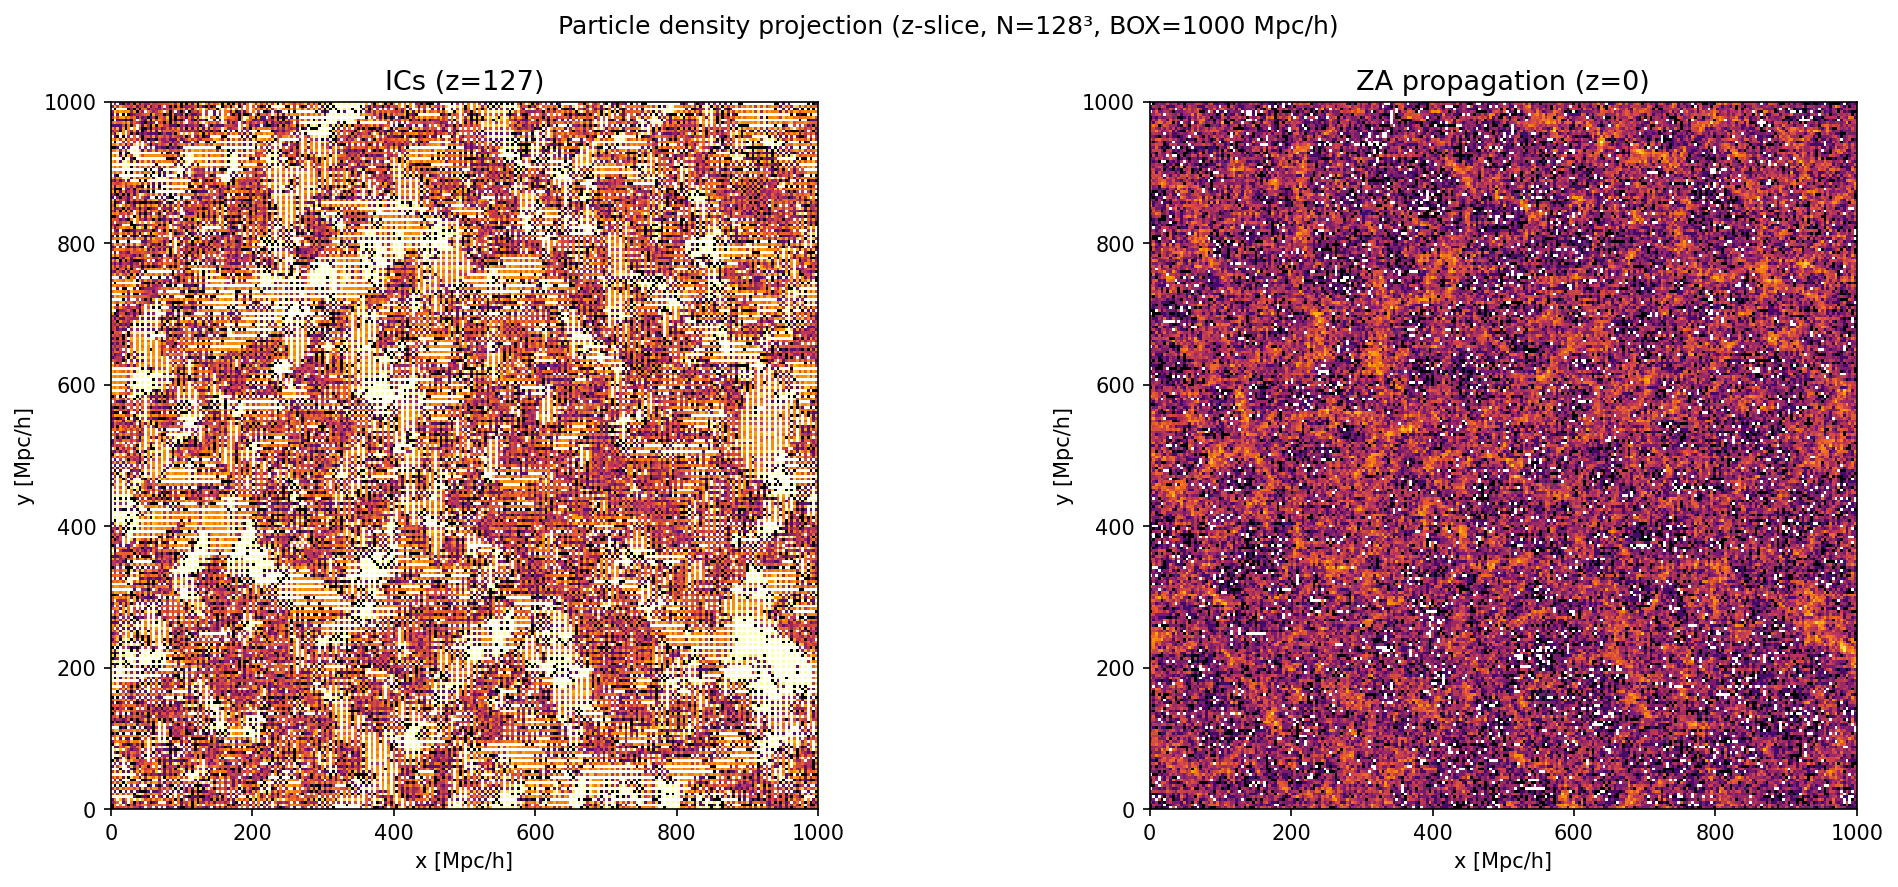
\includegraphics[width=0.5\textwidth]{../input_files/plots/density_projection.png}
    \caption{Projected particle density from a N=128³ simulation in a 1000 Mpc/h box, showing the initial conditions at z=127 (left) and their subsequent evolution to z=0 via the Zel'dovich Approximation (ZA) (right). The ZA propagation correctly transforms the nearly homogeneous initial state into the characteristic cosmic web structure, with clearly visible filaments, voids, and proto-cluster nodes.}
    \label{fig:image2}
\end{figure}

\section{Conclusions}
\label{sec:conclusions}


In this work, we addressed the significant computational cost associated with cosmological N-body simulations, a key bottleneck for generating the large statistical ensembles required by modern precision cosmology. We developed, benchmarked, and validated a GPU-accelerated Particle-Mesh (PM) simulation code built using the NVIDIA Warp framework, a Python-based toolkit for creating high-performance GPU kernels.

Our implementation simulates the gravitational evolution of $512^3$ particles. It leverages custom Warp kernels for the Cloud-in-Cell (CIC) mass assignment and force interpolation steps, and utilizes the cuFFT library for an efficient Fast Fourier Transform-based Poisson solver. We benchmarked this implementation against an equivalent multi-threaded CPU code and found a substantial performance increase. The GPU code achieved a total per-step speedup of 1,348$\times$, reducing the time for a single step from 89.4 seconds on the CPU to just 0.07 seconds on the GPU. The most dramatic gains were observed in the particle-grid interaction steps, which were accelerated by factors of over 2,000$\times$ and 9,000$\times$ for the mass deposit and force interpolation, respectively. This acceleration reduces the runtime of a typical 500-step simulation from over 12 hours to approximately 35 seconds.

We validated the physical fidelity of our pipeline by generating initial conditions at $z=127$ using the Zel'dovich Approximation and comparing the resulting matter power spectrum at $z=0$ against linear theory. The measured power spectrum agrees with the theoretical prediction from CAMB to within 4\% on large scales ($k < 0.04 \, h/\text{Mpc}$), confirming the accuracy of our initial condition generation and power spectrum estimation modules. Deviations on smaller scales, including a power deficit at intermediate scales and strong suppression at high $k$, are consistent with the known limitations of the Zel'dovich Approximation and are not indicative of flaws in the simulation code itself.

The primary conclusion of this study is that modern GPU programming frameworks like NVIDIA Warp provide an accessible and highly effective pathway for developing performant cosmological codes. The demonstrated speedup enables the rapid generation of mock universes, a critical capability for accurately estimating covariance matrices and interpreting data from large-scale structure surveys. This work successfully presents a validated, high-performance simulation tool that helps overcome a major computational challenge in contemporary cosmological research.


\bibliography{bibliography}{}
\bibliographystyle{unsrt}

\end{document}
